\documentclass[tikz,border=8pt]{standalone}
% Shared look for every TikZ diagram. Load with % Shared look for every TikZ diagram. Load with % Shared look for every TikZ diagram. Load with \input{../../tools/tikz-style.tex}
\usepackage[T1]{fontenc}
\usepackage{lmodern}
\renewcommand{\sfdefault}{lmr}  % diagrams use the same serif as the text
\usetikzlibrary{arrows.meta, positioning, shapes.geometric, calc, fit, backgrounds}
\definecolor{cblue}{HTML}{4C78A8}
\definecolor{corange}{HTML}{F58518}
\definecolor{cgreen}{HTML}{54A24B}
\definecolor{cred}{HTML}{E45756}
\definecolor{cpurple}{HTML}{B279A2}
\definecolor{cgrey}{HTML}{6B6B6B}
\tikzset{
  every picture/.style={font=\sffamily, line width=1.2pt},
  box/.style={draw=#1, fill=#1!12, rounded corners=4pt, align=center, inner sep=7pt, minimum height=1.1cm},
  box/.default=cgrey,
  arrow/.style={-{Stealth[length=3mm]}, draw=cgrey, line width=1.4pt},
  title/.style={font=\sffamily\bfseries\Large},
  note/.style={font=\sffamily\small, text=cgrey, align=center},
}
\AtBeginDocument{\hyphenpenalty=10000 \exhyphenpenalty=10000}

\usepackage[T1]{fontenc}
\usepackage{lmodern}
\renewcommand{\sfdefault}{lmr}  % diagrams use the same serif as the text
\usetikzlibrary{arrows.meta, positioning, shapes.geometric, calc, fit, backgrounds}
\definecolor{cblue}{HTML}{4C78A8}
\definecolor{corange}{HTML}{F58518}
\definecolor{cgreen}{HTML}{54A24B}
\definecolor{cred}{HTML}{E45756}
\definecolor{cpurple}{HTML}{B279A2}
\definecolor{cgrey}{HTML}{6B6B6B}
\tikzset{
  every picture/.style={font=\sffamily, line width=1.2pt},
  box/.style={draw=#1, fill=#1!12, rounded corners=4pt, align=center, inner sep=7pt, minimum height=1.1cm},
  box/.default=cgrey,
  arrow/.style={-{Stealth[length=3mm]}, draw=cgrey, line width=1.4pt},
  title/.style={font=\sffamily\bfseries\Large},
  note/.style={font=\sffamily\small, text=cgrey, align=center},
}
\AtBeginDocument{\hyphenpenalty=10000 \exhyphenpenalty=10000}

\usepackage[T1]{fontenc}
\usepackage{lmodern}
\renewcommand{\sfdefault}{lmr}  % diagrams use the same serif as the text
\usetikzlibrary{arrows.meta, positioning, shapes.geometric, calc, fit, backgrounds}
\definecolor{cblue}{HTML}{4C78A8}
\definecolor{corange}{HTML}{F58518}
\definecolor{cgreen}{HTML}{54A24B}
\definecolor{cred}{HTML}{E45756}
\definecolor{cpurple}{HTML}{B279A2}
\definecolor{cgrey}{HTML}{6B6B6B}
\tikzset{
  every picture/.style={font=\sffamily, line width=1.2pt},
  box/.style={draw=#1, fill=#1!12, rounded corners=4pt, align=center, inner sep=7pt, minimum height=1.1cm},
  box/.default=cgrey,
  arrow/.style={-{Stealth[length=3mm]}, draw=cgrey, line width=1.4pt},
  title/.style={font=\sffamily\bfseries\Large},
  note/.style={font=\sffamily\small, text=cgrey, align=center},
}
\AtBeginDocument{\hyphenpenalty=10000 \exhyphenpenalty=10000}

\begin{document}
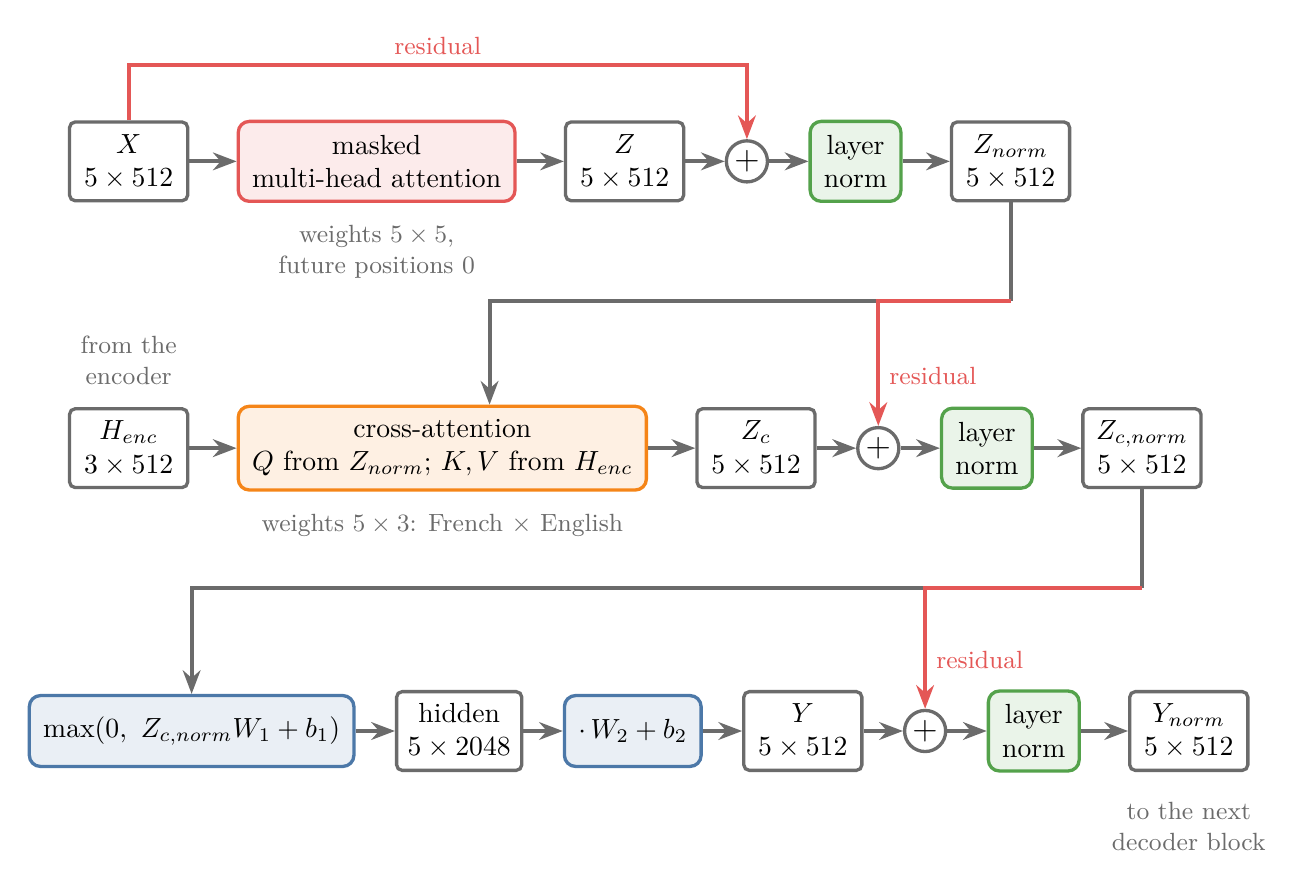
\begin{tikzpicture}[every node/.append style={font=\sffamily},
  mat/.style={draw=cgrey, fill=white, rounded corners=2pt, align=center, inner sep=4pt, minimum width=1.5cm, minimum height=1.0cm},
  op/.style={box=#1, inner sep=5pt, minimum height=0.9cm},
  plus/.style={draw=cgrey, circle, inner sep=1pt, font=\large}]
  % row 1: masked self-attention
  \node[mat] (X) at (0,0) {$X$\\$5 \times 512$};
  \node[op=cred, right=0.6cm of X] (mmha) {masked\\multi-head attention};
  \node[mat, right=0.6cm of mmha] (Z) {$Z$\\$5 \times 512$};
  \node[plus, right=0.5cm of Z] (p1) {$+$};
  \node[op=cgreen, right=0.5cm of p1] (ln1) {layer\\norm};
  \node[mat, right=0.6cm of ln1] (Zn) {$Z_{\text{norm}}$\\$5 \times 512$};
  \draw[arrow] (X) -- (mmha); \draw[arrow] (mmha) -- (Z); \draw[arrow] (Z) -- (p1); \draw[arrow] (p1) -- (ln1); \draw[arrow] (ln1) -- (Zn);
  \draw[arrow, draw=cred] (X.north) -- ++(0,0.7) -| node[pos=0.25, above, text=cred, font=\sffamily\small] {residual} (p1.north);
  \node[note, below=0.15cm of mmha] {weights $5 \times 5$,\\future positions 0};
  % row 2: cross-attention
  \node[mat, below=2.6cm of X] (H) {$H_{\text{enc}}$\\$3 \times 512$};
  \node[op=corange, right=0.6cm of H] (cross) {cross-attention\\$Q$ from $Z_{\text{norm}}$; $K, V$ from $H_{\text{enc}}$};
  \node[mat, right=0.6cm of cross] (Zc) {$Z_c$\\$5 \times 512$};
  \node[plus, right=0.5cm of Zc] (p2) {$+$};
  \node[op=cgreen, right=0.5cm of p2] (ln2) {layer\\norm};
  \node[mat, right=0.6cm of ln2] (Zcn) {$Z_{c,\text{norm}}$\\$5 \times 512$};
  \draw[arrow] (H) -- (cross); \draw[arrow] (cross) -- (Zc); \draw[arrow] (Zc) -- (p2); \draw[arrow] (p2) -- (ln2); \draw[arrow] (ln2) -- (Zcn);
  \coordinate (zdown) at ([yshift=-1.25cm]Zn.south);
  \draw[draw=cgrey, line width=1.4pt] (Zn.south) -- (zdown);
  \draw[arrow] (zdown) -| ([xshift=0.6cm]cross.north);
  \draw[arrow, draw=cred] (zdown) -| node[pos=0.8, right, text=cred, font=\sffamily\small] {residual} (p2.north);
  \node[note, below=0.15cm of cross] {weights $5 \times 3$: French $\times$ English};
  \node[note, above=0.15cm of H] {from the\\encoder};
  % row 3: feed-forward
  \node[op=cblue, below=2.6cm of H, xshift=0.8cm] (f1) {$\max(0,\ Z_{c,\text{norm}}W_1 + b_1)$};
  \node[mat, right=0.5cm of f1] (Hm) {hidden\\$5 \times 2048$};
  \node[op=cblue, right=0.5cm of Hm] (f2) {$\cdot\, W_2 + b_2$};
  \node[mat, right=0.5cm of f2] (Y) {$Y$\\$5 \times 512$};
  \node[plus, right=0.5cm of Y] (p3) {$+$};
  \node[op=cgreen, right=0.5cm of p3] (ln3) {layer\\norm};
  \node[mat, right=0.6cm of ln3] (Yn) {$Y_{\text{norm}}$\\$5 \times 512$};
  \coordinate (cdown) at ([yshift=-1.25cm]Zcn.south);
  \draw[draw=cgrey, line width=1.4pt] (Zcn.south) -- (cdown);
  \draw[arrow] (cdown) -| (f1.north);
  \draw[arrow, draw=cred] (cdown) -| node[pos=0.8, right, text=cred, font=\sffamily\small] {residual} (p3.north);
  \draw[arrow] (f1) -- (Hm); \draw[arrow] (Hm) -- (f2); \draw[arrow] (f2) -- (Y); \draw[arrow] (Y) -- (p3); \draw[arrow] (p3) -- (ln3); \draw[arrow] (ln3) -- (Yn);
  \node[note, below=0.25cm of Yn] {to the next\\decoder block};
\end{tikzpicture}
\end{document}
